\documentclass[a4paper, 12pt]{report}

% Adapté du tempate TER-M1 de l'Université de Paris

%%%%%%%%%%%%
% Packages %
%%%%%%%%%%%%

\usepackage[french]{babel}
%\usepackage{hyperref}
\usepackage[noheader]{packages/sleek}
\usepackage{packages/sleek-title}
\usepackage[french]{packages/sleek-theorems}
\usepackage{packages/sleek-listings}
\usepackage{tikz}
\usepackage[french,linesnumbered,lined]{algorithm2e}
\usepackage{pdfpages}
\usepackage[export]{adjustbox}[2011/08/13]
\SetKwInput{KwResult}{R\'esultat}
\SetKw{KwInput}{Entr\'ees}
%%%%%%%%%%%%%%
% Title-page %
%%%%%%%%%%%%%%

\logo{./resources/img/logo_science.png}
\institute{Sorbonne Université}
\faculty{Master ANDROIDE}
\title{Interaction Humain-Machine \& Sciences cognitives}
\subtitle{Étude sur la gratification différée - UE de projet M1}
\author{Éric \textsc{ZHANG} -- Kate \textsc{ZHANG}}
\date{2022}



%%%%%%%%%%%%%%%%https://www.overleaf.com/project/6012bd305aee4065605e8f1d
% Bibliography %
%%%%%%%%%%%%%%%%

\addbibresource{./resources/bib/references.bib}

%%%%%%%%%%
% Others %
%%%%%%%%%%

\lstdefinestyle{latex}{
    language=TeX,
    style=default,
    %%%%%
    commentstyle=\ForestGreen,
    keywordstyle=\TrueBlue,
    stringstyle=\VeronicaPurple,
    emphstyle=\TrueBlue,
    %%%%%
    emph={LaTeX, usepackage, textit, textbf, textsc}
}

\FrameTBStyle{latex}

\def\tbs{\textbackslash}

%%%%%%%%%%%%
% Document %
%%%%%%%%%%%%

\begin{document}
    \maketitle
    \romantableofcontents
    
    \chapter{Introduction}
    
    Notre projet vise à répondre à la question "Pourquoi ne devenons nous pas des experts ?" sur le sujet
    des systèmes interactifs.
    Cette question est légitime dans une multitude de contextes. 
    Pour une multitude de tâches qui sont quotidiennes pour beaucoup de personnes (traitement de texte, 
    montage photo/vidéo), il existe des outils qui sont faits pour les experts (LaTeX, Adobe Photoshop).
    Ces applications sont conçues avec le but de gagner en efficacité à travers différents vecteurs. Par 
    exemple à travers des raccourcis claviers \cite{remington2016practice} ou bien l’agencement des 
    éléments de l’interface graphique\cite{bailly2016visual,oulasvirta2018computational}.
    
    Malgré cela, il se trouve que les utilisateurs ne tirent pas avantage de ces améliorations qui font 
    pourtant l'essence de l'efficacité de l'outil de l’outil\cite{cockburn2014supporting}. Il s’agit d’une opposition 
    inattendue entre l’utilisateur qui choisit un outil pour son efficacité tout en ignorant les 
    fonctionnalités supplémentaires qui la proposent. À la place, les utilisateurs préfèrent se cantonner 
    aux fonctionnalités offertes au premier abord par l'outil, ils décident de rester des Novices.
    
    L’étude de ce paradoxe est au cœur de notre projet, et en particulier l’analyse de la barrière de
    l’apprentissage, le coût en temps posé par la tâche de la prise en main de ces fonctionnalités.
    
    
    En somme, l'objectif est d'identifier l'impact de la barrière de l'apprentissage sur les décisions de 
    l'utilisateur. Quels sont les facteurs qui motivent l'utilisateur à choisir une option au dessus d'un autre ? 
    Est-ce une décision faite de manière rationnelle ?
    
    En vue de cet objectif, la réalisation d'un dispositif permettant d'exposer et récolter 
    des données provenant d'utilisateurs réels est nécessaire. 
    
    
    Le projet est encadré par Gilles BAILLY, chercheur du CNRS dans le laboratoire de l'ISIR (Institut des 
    Systèmes Intelligents et de Robotique) spécialisé dans l'Interaction Humain-Machine.
    
    
    Le \href{https://github.com/KomeRice/temporal-discounting/tree/master}{code source du site web} est 
    accessible publiquement sur Github. 
    
    Le site web est actuellement hébergé par le laboratoire de l'ISIR à l'adresse: 
    
    \href{https://ihm-nodejs.isir.upmc.fr/}{https://ihm-nodejs.isir.upmc.fr/}
    
    
    \chapter{État de l'art}
    \textbf{Transition novice à expert}
    
    En interaction humain-machine, le mode Novice d'un système interactif est l'ensemble des interactions 
    par défaut, souvent visuels prévues pour les utilisateurs débutants afin de faciliter
    la prise en main d'une interface, comme des menus déroulants ou des icônes. 
    Le mode Expert est lui destiné à des utilisateurs avancés et peut se présenter par exemple
    sous la forme de raccourcis clavier ou des interactions gestuelles.
    
    La transition de novice à expert est un problème complexe qui comprend les notions d'apprentissage, de 
    prise de décision et de biais cognitifs.
    Des recherches \cite{carroll5} ont montré que même si les utilisateurs connaissent les avantages du 
    mode expert, ils ne vont pas nécessairement faire l'effort de consacrer du temps à apprendre. Et même
    après avoir pris en main le mode Expert, les utilisateurs sont 
    susceptibles d'oublier son utilisation.\cite{lafreniere2017investigating}.
    
    Des expériences\cite{augenblick2019experiment} et hypothèses\cite{lane2005hidden} ont déjà été 
    proposées pour expliquer ce phénomène, et quelques solutions ont été proposées pour par exemple
    régler le paradoxe de l'utilisateur actif.\cite{krisler2008training} C'est à dire le fait que les 
    utilisateurs favorisent la productivité à court terme au détriment de l'efficacité à long terme.
    
    \textbf{Gratification différée (Time Discouting)}
    
    La gratification différée est le concept de ne pas tirer avantage de bénéfices futurs en échange  
    d'avantages présents mais moindre en comparaison.
    Par exemple une personne aurait tendance à préférer recevoir 10 Euros aujourd'hui plutôt que 11 Euros 
    le jour ou l'année suivante.\cite{frederick2002time}.
    Ce concept a déjà été étudié en profondeur dans le domaine de l'économie 
    \cite{chapman1996temporal,chapman1995valuing,green1997rate} et de la 
    psychologie\cite{ainslie1975specious} et intervient fréquemment dans la vie quotidienne, que ce soit 
    pour la procrastination\cite{fischer2001read}, ou pour d'autres choix du quotidien 
    \cite{baker2003delay}.
    
    Le but de notre projet de d'appliquer le concept de gratification différée sur le domaine de 
    l'interaction humain-machine plus particulièrement sur la transition novice-expert.
    Pour voir si nous pouvons expliquer l'irrationalité des utilisateurs par la gratification différée. Ces principes sont le plus souvent mis en évidence à travers une échelle plus large, de plusieurs jours ou plusieurs mois. Nous étudions ce phénomène à une échelle plus locale de quelques minutes.
    
    \chapter{Contribution}
    L'expérience étudiée est décrite dans ce papier\cite{bailly} fourni par notre professeur encadrant. 
    \section{Modélisation}
        \subsection{Présentation de l'interface}
        Dans le but de pouvoir réaliser un système supportant une expérience distribuable à des utilisateurs facilement, la solution d'un site web a été retenue.
        
        L'interface se décline en plusieurs éléments:
        \begin{figure}[H]
            \centering
            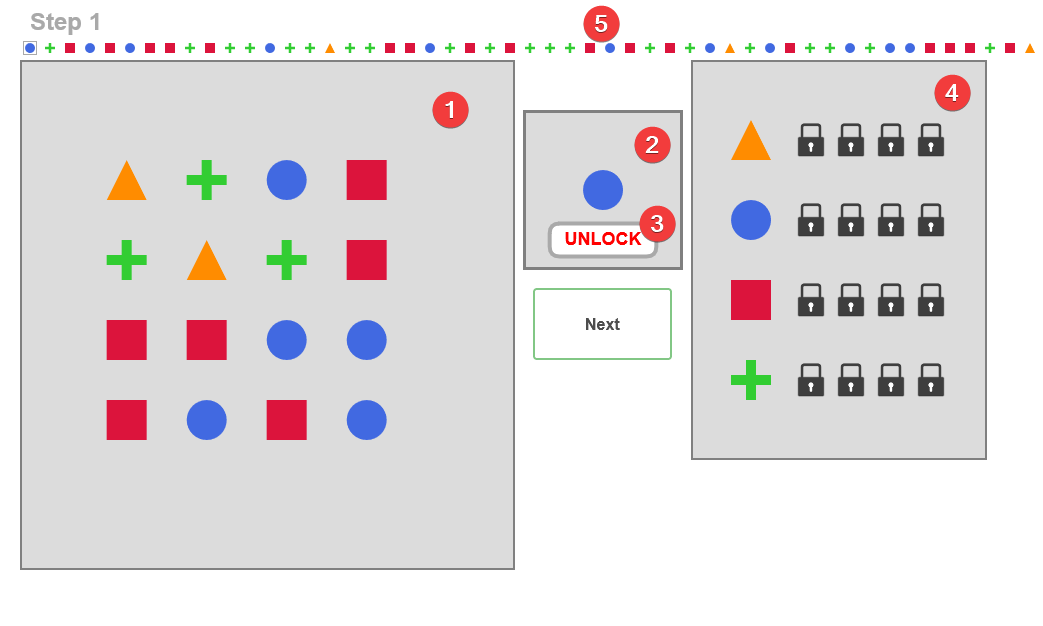
\includegraphics[width=1\textwidth]{img/annotedScreen.png}
            \noskipcaption{Interface de jeu}
        \end{figure}
        
        
        \begin{description}
            \item[(1) Grille de jeu] Contient les formes à sélectionner parmi d'autres formes aléatoires
            \item[(2) Panel cible] Affiche la forme cible de l'essai courant
            \item[(3) Bouton déverrouillage] Un bouton qui une fois cliqué révèle l'interaction à effectuer pour déverrouiller un cadenas pour une forme
            \item[(4) Panel d'apprentissage] Montre le nombre de cadenas déverrouillé pour chaque forme ainsi que le nombre de cadenas restants
            \item[(5) Frise temporelle] Indique les formes prochaines
        \end{description}
        
        \begin{figure}[H]
            \centering
            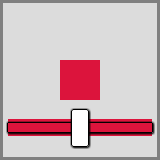
\includegraphics[width=0.2\textwidth]{img/unlockTask.png}
            \noskipcaption{Tâche de déblocage}
        \end{figure}
        
        Une fois les formes sélectionnées, l'utilisateur peut opter pour utiliser le mode Apprentissage
        (ici simulé par une petite tâche ayant une durée fixe pour l'essai) afin de pouvoir
        graduellement débloquer le mode Expert. L'utilisateur doit faire des aller-retours avec
        le curseur pendant un certain temps afin de pouvoir compléter la tâche.

        \subsection{Déroulement du jeu}
        Pour modéliser le passage du mode novice au mode expert, nous avons suivi les consignes du papier\cite{bailly}.
        Nous avons donc trois modes :
        \begin{itemize}
            \item Le mode Novice : l'utilisateur sélectionne toutes les instances d'une forme cible et clique sur "Suivant" ("Next") pour passer à la prochaine grille. Ce mode représente les manipulations de l'utilisateur lorsqu'il souhaite faire une commande sur un système interactif.
            \item Le mode Expert : débloqué lorsque l'utilisateur a ouvert tous les verrous d'une forme, il 
            n'a plus qu'à cliquer sur une seule instance et toutes les instances seront automatiquement sélectionnées. Il peut ensuite cliquer sur le bouton "Suivant" ("Next"). Ce mode correspond au moment où l'utilisateur est à l'aise avec les commandes expertes du système.
            \item Le mode Apprentissage : l'utilisateur sélectionne toutes les instances d'une forme cible puis clique 
            sur un bouton "Déverrouiller" ("Unlock"), il doit ensuite agiter une barre de défilement pendant un certain temps $T_{slider}$ et cliquer sur "Suivant" ("Next") pour ouvrir un verrou. 
            Ce mode correspond aux manipulations qu'il fait lorsqu'il souhaite apprendre à utiliser les raccourcis du système interactif. Lui et le temps minimum passé dessus représentent la barrière de l'apprentissage.
        \end{itemize}
        
        Pour une bonne modélisation, il faut alors que le mode apprentissage soit plus long que le mode novice et le mode expert soit le plus rapide de tous les modes.
    
        Le temps novice et le temps expert sont influencés par les paramètres de l'expérience.
        Le temps d'apprentissage, lui est l'aspect le plus important de l'expérience. Car on veut savoir si, 
        avec un même temps d'apprentissage, comment le nombre de verrous va affecter le choix de 
        l'utilisateur.
        
        L'utilisateur se voit donc proposé d'abord une série de trois tutoriels, présentant les trois modes
        utilisables dans le jeu: Le mode Novice, le mode Expert et le mode Apprentissage.
        
        Une fois les tutoriels passés, l'utilisateur commence l'expérience. Un chronomètre caché est lancé
        et l'utilisateur doit compléter le plus d'essais dans le temps imparti. Les essais
        sont générées à l'infini et l'utilisateur doit alors mettre en œuvre les mécaniques
        apprises dans les tutoriels. 
        
        En plus du nombre de verrous, nous ajoutons un autre paramètre, la fréquence des formes, qui va 
        représenter la fréquence d'utilisation des commandes. Ainsi une commande peu utilisée sera modélisée 
        par une fréquence plus faible. Ce paramètre va nous permettre de différencier les cas ou l'utilisateur va 
        décider d'apprendre.
        
        Chaque forme ayant une fréquence, les essais sont générés par blocs pour garantir l'apparition de certaines 
        formes à certains intervalles. 
        Chaque bloc comporte un nombre d'essais égal à la fréquence de chaque forme. Ainsi pour 
        quatre formes de fréquence respectives (1, 2, 3, 4), un bloc de 10 essais sera généré,
        chaque forme ayant un essai par unité de fréquence. Le bloc est ensuite mélangé et ajouté
        à une queue qui est défilée à chaque fois que l'utilisateur complète un essai.
        
        Des pauses régulières sont proposées, et une fois le temps écoulé, les 
        données sont enregistrées et l'utilisateur a la possibilité de donner son avis afin de 
        potentiellement améliorer l'expérience.
        
        \subsection{Choix des paramètres}

        Nos paramètres sont donc : Le temps d'apprentissage total, les fréquences des différentes formes et le nombre de verrous pour chacunes d'elles. 
        Nous souhaitons mesurer le temps mis par l'utilisateur pour passer un essai, et quand il décide à passer au mode expert.
        
        Nous avons donc choisi arbitrairement un temps d'apprentissage total d'une minute, c'est à dire 
        que peu importe les autre paramètres, il faut exactement une minute pour débloquer le mode expert 
        pour une forme.
        
        Pour la fréquence des verrous, nous avons étudié plusieurs cas théoriques et avons choisi les 
        fréquences 1, 4, 6 et 8.
        C'est à dire que pour chaque apparition de la forme de fréquence 1 il y aura 8 apparitions de la forme de fréquence 8.
        
        Cela force l'utilisateur a évaluer l'avantage de débloquer une forme, en effet plus une formes est
        commune plus débloquer le mode Expert pour elle rapporte en gain de temps. À l'inverse, débloquer
        le mode Expert pour les formes plus rares peut s'avérer être une perte de temps.
        
        \begin{figure}[H]
            \centering
            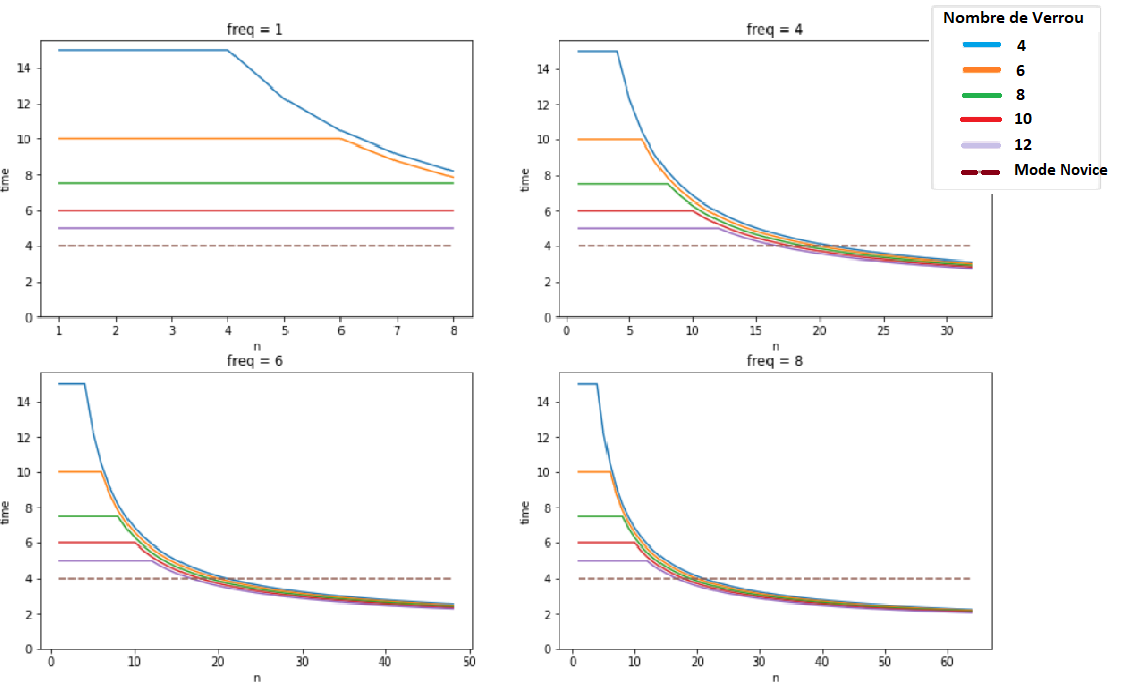
\includegraphics[width=0.9\textwidth]{img/fig3.png}
            \caption{Évolution théorique du temps moyen en fonction du nombre d'épreuve, si l'utilisateur n'utilise que le mode expert}
        \end{figure}
        
        Ici, il n'y a pas d'avantage à débloquer la forme de fréquence 1. Pour celle de fréquence 4, le 
        résultat est un peu plus rapide si les utilisateurs déverrouillent mais c'est assez négligeable. Enfin pour les formes de fréquence 6 et 8, 
        l'utilisateur gagne du temps à les débloquer.
        
        Remarque: Si l'utilisateur est rapide, il pourrait potentiellement obtenir un gain en temps
        si il décide de débloquer la forme de fréquence 4, celle de fréquence 1 toutefois
        restera désavantageuse à débloquer.
        
        \begin{figure}[H]
            \centering
            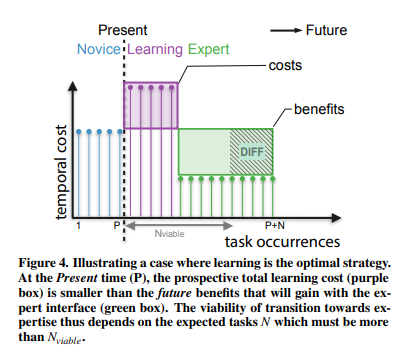
\includegraphics[width=0.5\textwidth]{img/fig2.png}
            \caption{Figure dans le papier présentant un cas où il est avantageux de débloquer}
        \end{figure}
        
        Enfin pour le nombre de verrous, dans un premier temps nous les avions choisi arbitrairement.
        
        Une condition d'arrêt était nécessaire pour l'expérience : limiter le nombre de essais 
        maximum était préconisé tout en encourageant l'utilisateur à aller le plus vite possible. 
        Ainsi, nous avions suivi ce qui était écrit et avons délimité l'expérience par un nombre d'essais maximal.
        
        \begin{figure}[H]
            \centering
            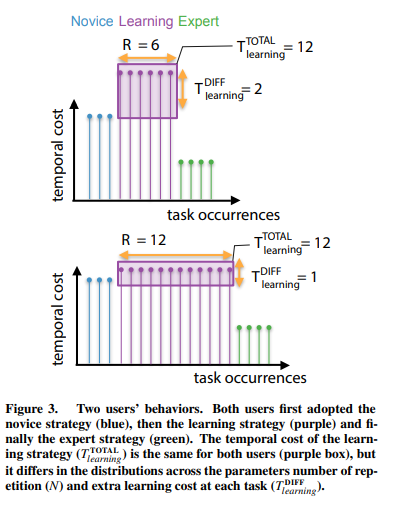
\includegraphics[width=0.5\textwidth]{img/fig1bad.png}
            \noskipcaption{Hypothèse initiale sur la répartition du temps d'apprentissage}
        \end{figure}
        
        Mais on s'est rendu compte que cette condition ne convenait pas, car cela pénalisait les 
        configurations avec un grand nombre de verrous. Car sachant que le temps d'apprentissage est 
        identique, et que le nombre d'essais est constant, nous avions moins d'utilisations du mode 
        expert dans les configurations avec un grand nombre de verrous que dans les configurations avec un 
        petit nombre.
        
        Nous avons donc décidé de changer la modalité de la condition d'arrêt, et de mettre un temps 
        limite de 10 minutes à la place. Dans ce laps de temps, l'utilisateur doit compléter le plus d'essais possible. 
        
        Nous avions dû donc adapter le nombre de verrous $R$ pour correspondre aux calculs suivants 
        
        $T_{learningTotal} = T_{learningUnique} * R$ et 
        
        $T_{learningUnique} = T_{novice} + T_{diff}$
        
        Alors afin d'éviter d'avoir une tâche de déverrouillage à durée négative, nous avons choisi 4, 6, 8, 10 et 12 verrous.
        
        \begin{figure}[H]
            \centering
            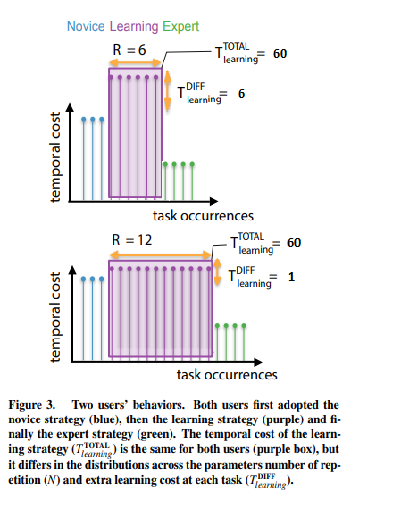
\includegraphics[width=0.5\textwidth]{img/fig1.png}
            \noskipcaption{Graphe après le changement}
        \end{figure}
       
        Là, on obtient bien des configurations équitables, et il nous restait plus qu'à 
        faire passer des utilisateurs réels et d'analyser les résultats.
    
        \section{Implémentation}
        Le site web est réalisé à l'aide de HTML pour donner la forme du site web,
        Javascript pour gérer les interactions et utilise des feuilles CSS pour contrôler le style de la page.
        
        
        Toutefois ces technologies s'exécutent intégralement sur le côté client de l'utilisateur, c'est-à-dire 
        son navigateur. Afin de pouvoir capturer et sauvegarder les métriques primordiales à notre recherche
        ainsi que d'assurer une distribution égale des modalités sur l'ensemble des utilisateurs,
        une technologie s'exécutant du côté serveur est nécessaire.
        Node.js est le moteur qui permet la gestion de ces éléments, permettant ainsi de maintenir un serveur
        capable d'enregistrer les données envoyées par le navigateur de l'utilisateur.
        
        
        Le code source est initialement basé sur le travail réalisé par des étudiants de Sorbonne Université 
        pour l'UE de Projet sur le même sujet.
        
        \subsection{Réécriture}
        Le code initial a été difficile à prendre en main, et il était compliqué pour nous d'identifier 
        exactement où et comment les différentes étapes du jeu étaient mises en place. Dans le 
        but de nous faciliter l'ajout de potentiels nouveaux composants ou la modification 
        de la logique existante, nous avons décidé de réécrire la majorité du code existant.
        
        Un des objectifs étant d'établir une structure plus succincte représentant où les
        fonctions du jeu et les composants individuels sont identifiables avec un fonctionnement
        plus indépendant que précédemment. Cela nous a également permis de mieux nous familiariser
        avec l'architecture d'un site web dynamique et plus précisément avec le Javascript.
        
        En particulier, le code initial utilisait un module Node.js nommé "nedb" afin de pouvoir gérer 
        les paramètres du jeu et la sauvegarde des données utilisateur. Ce module n'est néanmoins plus
        maintenu depuis plus de 5 ans \href{https://www.npmjs.com/package/nedb}{(Dernière mise à jour le 15 Février 2016 sur 
        npm, le gestionnaire de paquets de Node.js)}. Cela signifie donc que le module n'a plus reçu de 
        mises à jour de sécurité de ce moment là. Il se trouve qu'une faille de sécurité a été découverte et publiée
        le 15 Juin 2021 (\href{https://nvd.nist.gov/vuln/detail/CVE-2021-23395}{CVE-2021-23395}). 
        
        Cette vulnérabilité nommée \verb+Prototype Pollution+ permettrait de potentiellement modifier des propriétés de 
        la classe générique \verb+Object+ de Javascript, causant ainsi un déni de service en redéfinissant 
        par exemple la valeur retournée par \verb+Object.prototype.toString+ pour être un nombre entier, faisant 
        ainsi planter le serveur. Cette faille peut aussi être escalader en exécution arbitraire de code 
        dans le cas où un attribut était évalué. Une des dépendances de "nedb" nommée "underscore" est également vulnérable à des injections arbitraires de code 
        (\href{https://nvd.nist.gov/vuln/detail/CVE-2021-23358}{CVE-2021-23358}).
        
        Le module a donc été remplacé par un fichier CSV où les données sont écrites avec le module 
        standard "fs" de Node.js.
        
        Tout d'abord, le code portant sur les composants graphiques du jeu sont séparés des fonctions 
        exécutant la logique du jeu. 
        Les différents composants du jeu ainsi que leurs propriétés sont séparés. 
        Chaque élément peut donc opérer indépendemment des autres.
        Le fichier principal contenant précédemment l'intégralité du code contient simplement 
        l'initialisation et la liaison des composants.
        
        Ainsi il est possible de centraliser la prise de statistiques à la portion du code gérant la logique du jeu.

    
    \section{Résultats et analyse}
    Les résultats que nous avons récolté sont sous format CSV et contiennent une variété de métriques comme:
    \begin{itemize}
        \item Nombre d'essais complétés
        \item Mode utilisé pour chaque essai
        \item Temps passé sur chaque essai
    \end{itemize}
    
    Nous avons ensuite utilisé Jupyter Notebook et des outils comme Pandas et Seaborn pour faire l'analyse.
    Nous avions écrit un Notebook où toute la visualisation est automatique des lors que l'on fournit la base de données
    
        \subsection{Mise en place de l'expérience}
        Avant de commencer l'expérience, nous avons dû estimer le temps que l'utilisateur va prendre dans 
        chaque mode. Nous avons donc fait passer quelques utilisateurs sur le site avec pour but de mesurer le temps en mode novice, en mode apprentissage et en mode expert.
        
        \begin{figure}[H]
            \centering
            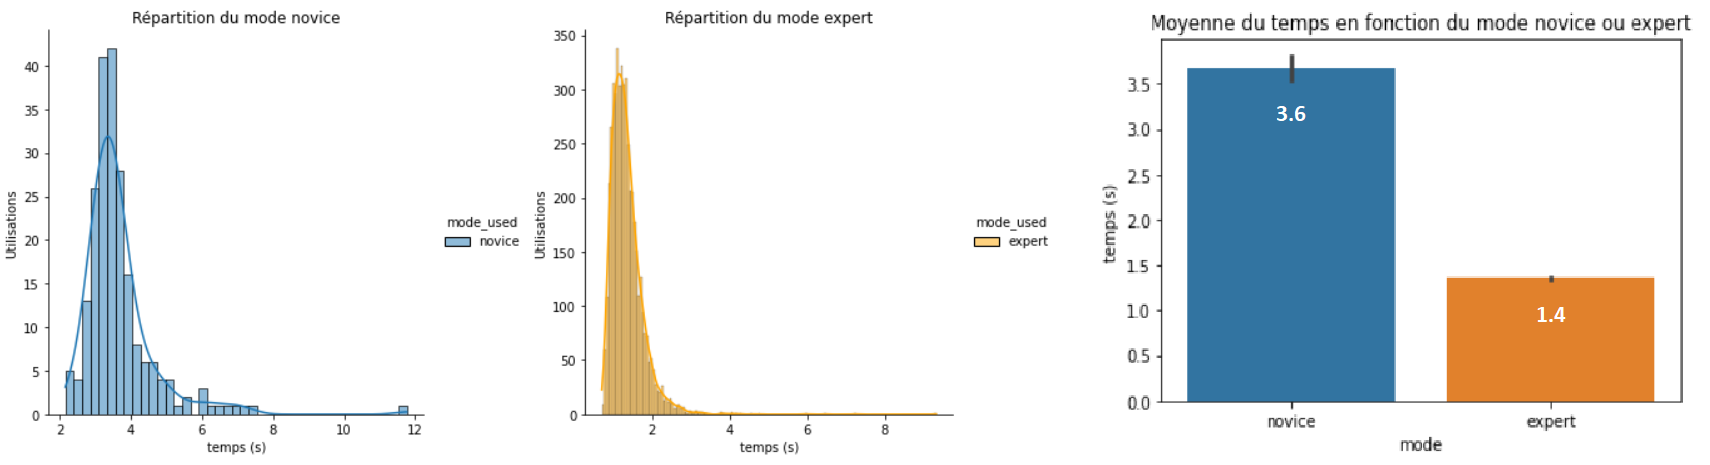
\includegraphics[width=0.9\textwidth]{img/fig4.png}
            \caption{Répartition du temps des utilisateurs dans les modes novice et expert}
        \end{figure}
        
        Nous avons donc mesuré (population jeune et dans le domaine de l'informatique) un temps moyen de 
        3,6s en mode novice et 1.4s en mode expert.
        
        Ensuite il était nécessaire de vérifier que nos temps d'apprentissage correspondaient bien 
        aux temps voulu.
        \begin{figure}[H]
            \centering
            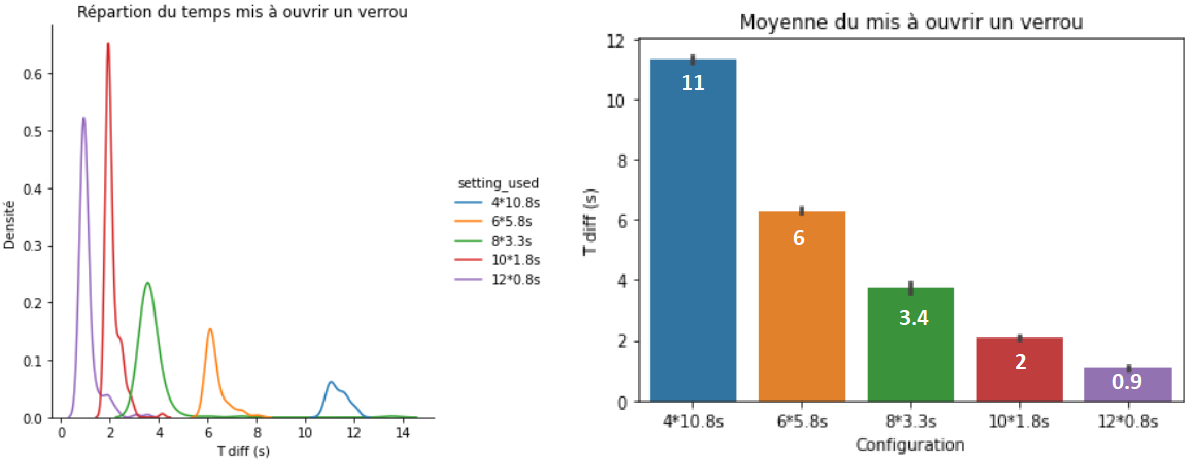
\includegraphics[width=1\textwidth]{img/fig5.png}
            \caption{Répartition du temps des utilisateurs dans le mode apprentissage}
        \end{figure}
        
        Nous obtenons des temps un peu au dessus de nos paramètres, nous avons alors réduit 
        artificiellement de 0.1s la durée de la tâche de déverrouillage.
        Toutefois même avec cet ajustement, en fonction de l'utilisateur, la variance entre les utilisateurs peuvent aller jusqu'à 2 secondes.
        
        \subsection{Résultats théoriques}
        Notre hypothèse est que les utilisateurs ne sont pas rationnels et ne feront pas les choix 
        optimaux pour aller le plus vite possible. Sous cette hypothèse, puisque le temps 
        d'apprentissage est le même peu importe le nombre de verrous, le temps passé à compléter les 
        essais sera alors le même pour chaque fréquence.
        Et donc voila le graphe théorique si les utilisateurs ne débloquent qu'une fréquence.
        Alors, si l'utilisateur ne débloque qu'une seule des formes, le graphe du temps passé devrait
        avoir l'allure suivante:
        
        \begin{figure}[H]
            \centering
            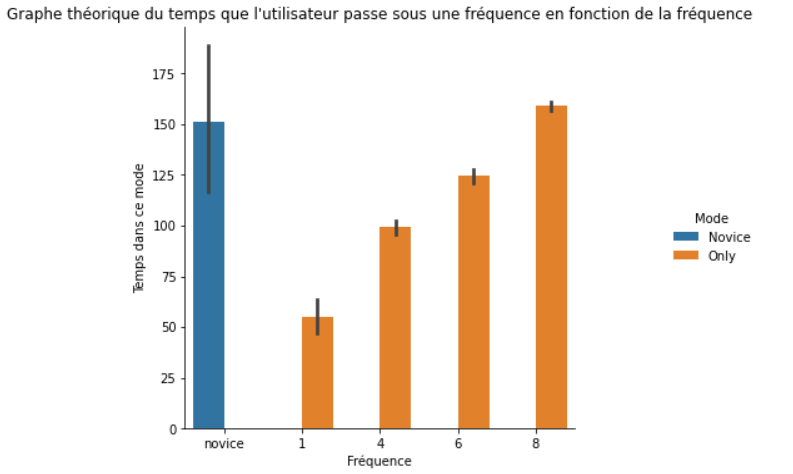
\includegraphics[width=0.8\textwidth]{img/fig6.png}
        \end{figure}
        
        Nous avons déterminé que pendant le temps imparti de 10 minutes, les utilisateurs sont en moyenne
        capable de faire 8 blocs en utilisant seulement le mode Novice, et 14 blocs en utilisant
        le mode Expert.
        
        Donc si les utilisateurs sont rationnels, ils débloqueront dès le départ les formes de 
        fréquences 4, 6 et 8 et compléter environ 14 blocs, soit 280 essais.
        
        \subsection{Résultats expérimentaux}
        Un total de 20 utilisateurs ont participé à notre expérience, ils ont été réparti du mieux 
        possible sur chacunes des conditions.
        
        Voici le graphe obtenu expérimentalement comparant pour chaque forme le temps passé dans chacun
        des modes. Il était attendu pour chaque fréquence un temps d'utilisation similaire. 
        C'est le cas ici, mais toutefois on voit que toutes les mesures prises sont supérieures à 
        celles obtenues par la théorie (Car les utilisateurs ne déverrouillent pas qu'un seul verrou), 
        même pour la forme de fréquence 1 qui représente pourtant une perte de temps. 
        On remarque également une grande variance sur les conditions avec des verrous plus long, une 
        base d'utilisateur plus grande pourrait minimiser cet effet car chaque configuration 
        a en moyenne 4 cas d'études.
        
        \begin{figure}[H]
            \centering
            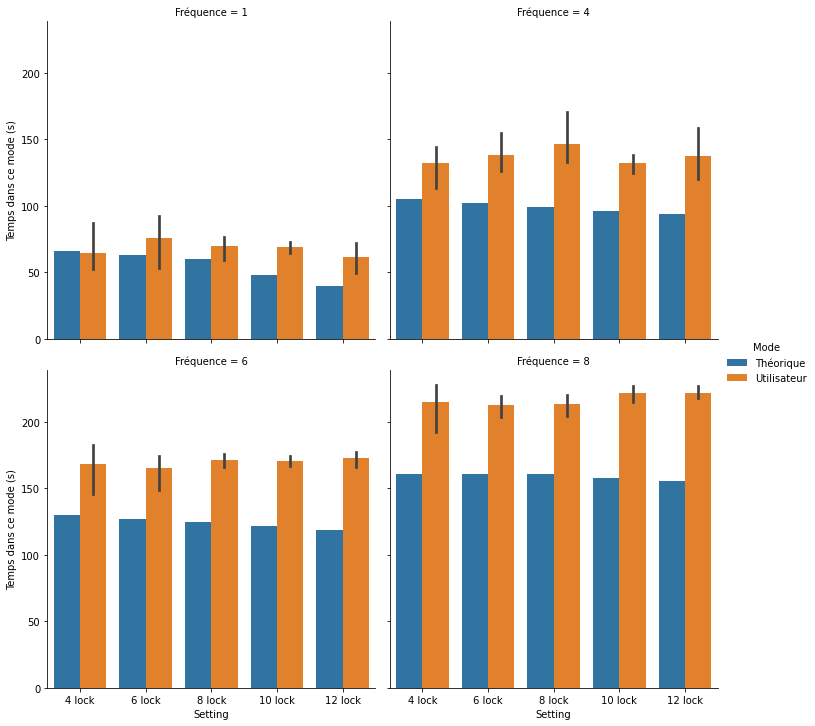
\includegraphics[width=1\textwidth]{img/fig7.png}
            \caption{Graphe du temps que l'utilisateur passe sous une fréquence en fonction du nombre de verrous}
        \end{figure}
        
        Sur cette figure portant sur le nombre de verrous ouvert a la fin de l'expérience, on observe que pour toute les configuration de verrous un schéma semblable pour les formes de fréquence 6 et 8, les verrous ont tous été ouverts. 
        Pour 4, il y a eu des hésitations, certains l'on débloqué autres non.
        Par contre pour la fréquence 1, on a différentes situations : Certains utilisateurs décident
        de ne pas déverrouiller le mode Expert tandis que d'autres le font alors que cela ne leur est pas avantageux.
        Cela montre un comportement irrationnel de l'utilisateur.
        
        \begin{figure}[H]
            \centering
            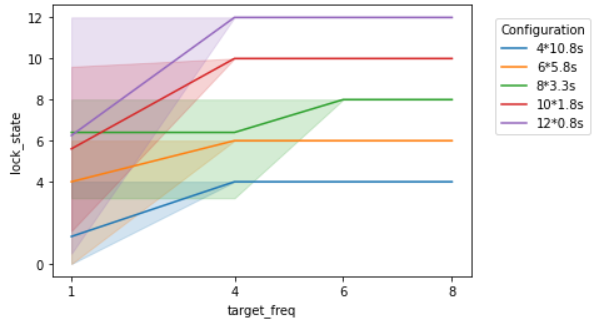
\includegraphics[width=0.8\textwidth]{img/fig8.png}
            \caption{Nombre de verrous ouvert à la fin de l'expérience en fonction de la fréquence de la forme}
        \end{figure}
        
        Sur cette figure, nous observons que les utilisateurs recherchent l'accès au mode Expert le
        plus rapidement possible. Donc le nombre de verrous déverrouilles augmente jusqu'à ce que
        le mode Expert soit débloqué. On voit donc que sur toutes les configurations des verrous
        les formes de fréquence 6 et 8 ont toujours été déverrouillé. 
        
        La plupart des utilisateurs ont décidé de déverrouiller le mode Expert pour la forme de fréquence 
        4, à gain nul ou moindre. 
        
        Toutefois, certains utilisateurs décident de débloquer le mode Expert pour la forme de fréquence 1 
        sans se rendre compte qu'il s'agit d'une perte de temps.
        
        \begin{figure}[H]
            \centering
            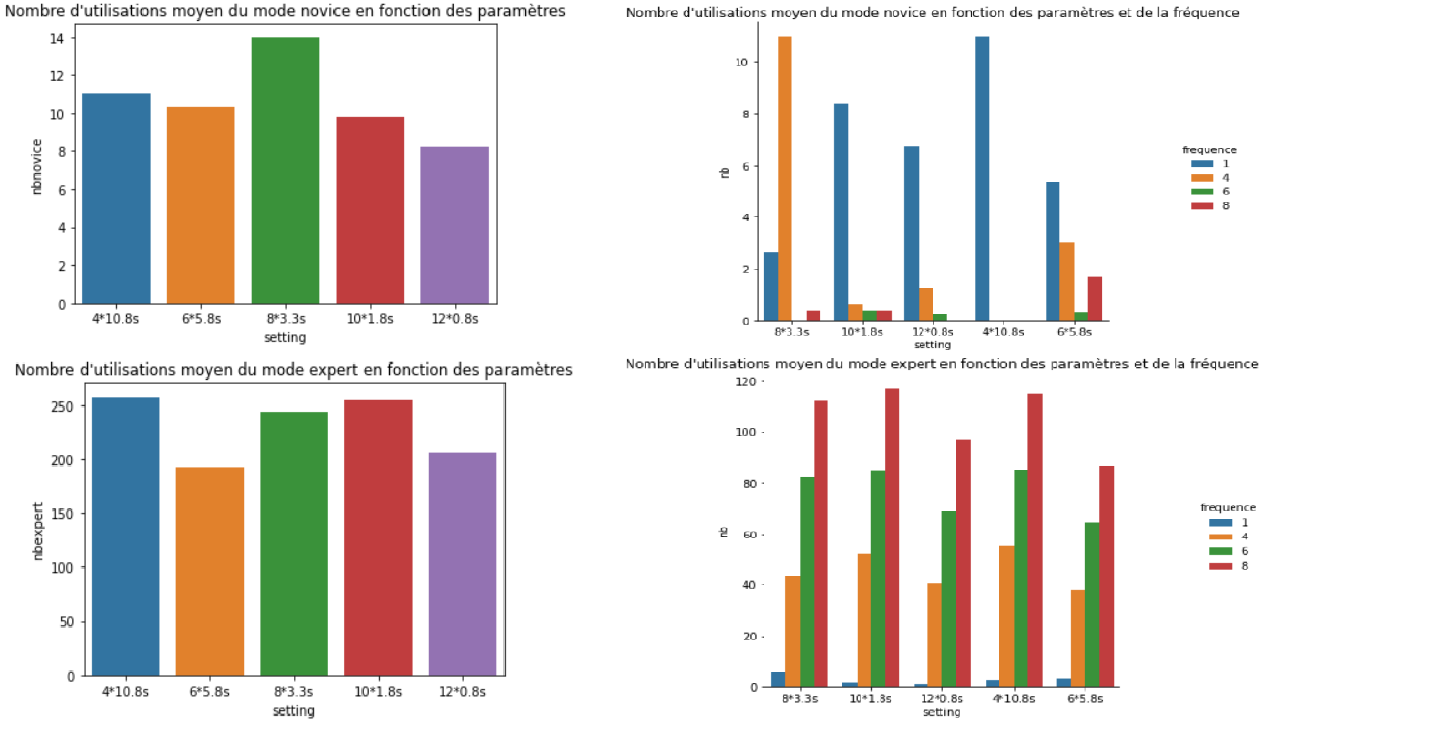
\includegraphics[width=0.8\textwidth]{img/fig9.png}
            \caption{Utilisation moyenne des modes novices et experts de nos utilisateurs}
        \end{figure}
        
        Enfin nous remarquons que certaines personnes commencé a déverrouiller pour une forme
        sans arriver au bout, s'arrêtant en cours de chemin ainsi que des utilisateurs qui entre deux
        ouvertures font une épreuve en mode novice.
        
        \begin{figure}[H]
            \centering
            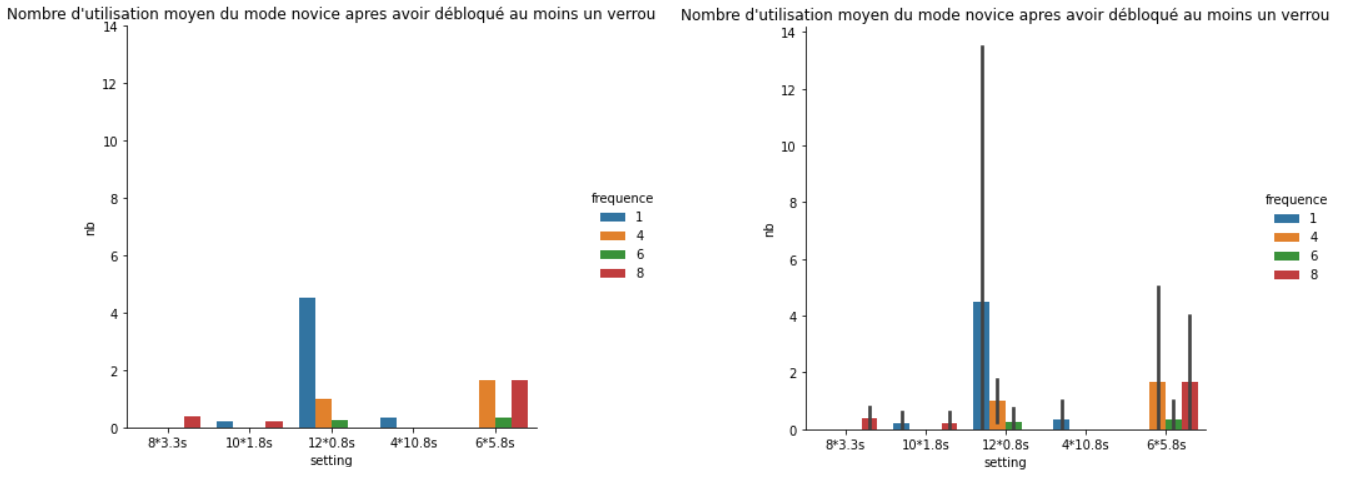
\includegraphics[width=1\textwidth]{img/fig10.png}
            \caption{Nombre d'utilisations du mode Novice après avoir ouvert au moins un verrou}
        \end{figure}
        
        En somme, nous pouvons souligner quelques comportements irrationnels des utilisateurs.
        Parfois oubliant de continuer à déverrouiller ou ne considérant pas la perte de temps à
        déverrouiller le mode Expert pour les formes à fréquence d'apparition faible.
        
    
    \chapter{Conclusion}
    Notre expérience a pu souligner des irrationalités auprès des utilisateurs. Parfois décidant
    de prendre des décisions allant à l'encontre de leur intérêt.
    
    Une étude plus compréhensive aurait pu être possible avec significativement plus d'utilisateurs
    que nous avions. De plus, les données que nous avons mesuré ne s'alignent parfois pas
    exactement avec les mesures théoriques. Il a également été nécessaire de changer la
    manière dont l'expérience était réalisée et l'utilisation de technologies étrangères qui
    ont prouvés être des obstacles chronophages.
    Nous n'avons pas pu plus exploiter tous nos métriques et d'autres hypothèses sont formulables.
    
    Néanmoins le prototype final est fonctionnel et modulable, il serait possible de mieux souligner la barrière de l'apprentissage avec plus d'utilisateurs et des paramètres plus précis.
    
    \section{Remerciements}
    Nous tenons à remercier spécialement notre encadrant Monsieur Gilles BAILLY pour son aide et sa grande implication durant tout le semestre pour ce projet, en particulier pour pour ses conseils qui nous a énormément servi dans nos moments de doutes.
    
    Nous tenons aussi à remercier tous les utilisateurs d'avoir dédié leur temps à tester notre prototype et de nous 
    permettre de collecter des données sur eux pour notre projet.

    
    \printbibliography

    \appendix
        \chapter{Cahier des charges}
        
\includepdf[pages=-]{cdc.pdf}
        
        \chapter{Manuel utilisateur}

        \section{Prérequis}
        \begin{itemize}
            \item Navigateur web (De préférence Mozilla Firefox, Google Chrome ou navigateur fondé sur Chromium)
            \item Git
            \item Node.js v16.14.2
        \end{itemize}
        \section{Mise en place}
        Le code est disponible à l'adresse: 
        
        
        \href{https://github.com/KomeRice/temporal-discounting}{https://github.com/KomeRice/temporal-discounting}
        
        
        Une copie du dépôt Git peut être téléchargée en entrant la commande suivante dans un terminal:
        
        \begin{verbatim}
        git clone https://github.com/KomeRice/temporal-discounting.git
        \end{verbatim}
        
        Installation de modules Node.js:
        \begin{verbatim}
        cd temporal-discounting/app
        npm install
        cd myexpress-init
        npm install
        \end{verbatim}
        
        Lancer le serveur Node.js (À exécuter depuis l'intérieur du dossier "app"à:
        \begin{verbatim}
        npm start
        \end{verbatim}
        
        
        Une fois le serveur lancé, une version locale du site web devrait être accessible à l'adresse:
        \href{http://localhost/}{http://localhost/}
        
        Les instructions pour prendre en main l'expérience sera affichée en tant que page d'accueil.
        
        Alternativement, un serveur hébergeant le site se situe à l'adresse:
        
        \href{https://ihm-nodejs.isir.upmc.fr/}{https://ihm-nodejs.isir.upmc.fr/}
        \section{Configuration et mesures}
        \subsection{Paramètres}
        Le fichier de configuration par défaut est situé dans "testSettings/testSettings.json". 
        L'emplacement de ce fichier peut être changé dans "app/rsc/assets/js/main.js@36" - Variable \verb+path+. 
        Il s'agit d'un objet JSON (JavaScript Object Notation).
        
        Les paramètres du jeu sont ainsi:
        \begin{description}
            \item[triWeight] Fréquence du triangle (int)
            \item[cirWeight] Fréquence du cercle (int)
            \item[squWeight] Fréquence du carré (int)
            \item[croWeight] Fréquence de la croix (int)
            \item[nbTargets] Nombre de formes cible à générer (int)
            \item[timeLearning] Temps d'apprentissage en ms (int)
            \item[nbSliders] (Fragment de l'ancien code, inutilisé) (int)
            \item[nbLocks] Liste des nombres de verrous possibles (list[int])
            \item[gridWidth] Largeur de la grille en nombre de formes (int)
            \item[gridHeight] Hauteur de la grille en nombre de formes (int)
            \item[shapeNames] Nom des formes (Changement découragé) (list[string])
            \item[showTimeline] Décide si la frise devrait être affichée (boolean)
            \item[easyMode] Décide si un clic dans le rectangle contenant la forme est toléré (boolean)
            \item[maxStep] Nombre d'essais maximum (-1 si infini) (int)
            \item[maxTimer] Durée maximale de l'expérience en ms (-1 si infini) (int)
            \item[noviceTime] Offset pour la définition de la durée du déverrouillage en ms (int)
            \item[breakTimer] Délai avant le début d'une pause en ms (int)
            \item[debug] Affiche des détails pour le débugging à l'écran (boolean)
        \end{description}
        
        \subsection{Données}
        Les données sont sauvegardées au format CSV dans "rsc/data/gameData.csv". 
        Chaque ligne correspond à une étape complétée par un utilisateur.
        
        Les données sauvegardées sont ainsi:
        \begin{description}
            \item[date] Date local du début de l'expérience
            \item[user\_ip] Addresse IP de l'utilisateur
            \item[trial\_id] Numéro de l'essai de la ligne
            \item[block\_id] Numéro du bloc de la ligne
            \item[n\_trials] Nombre d'essais complétés à la fin de l'expérience
            \item[n\_block] Nombre de blocs complétés à la fin de l'expérience
            \item[block\_size] Taille d'un bloc
            \item[target\_shape] Cible de l'essai courant
            \item[target\_id] ID de la forme cible
            \item[target\_freq] Fréquence de la forme cible
            \item[target\_n] Nombre de formes cible sur la grille
            \item[timeLearning] Temps d'apprentissage en ms
            \item[setting\_used] Nombre de verrous * Durée d'un verrou individuel
            \item[n\_locks] Nombre de verrous par forme
            \item[lock\_duration] Durée d'un verrou
            \item[unlock\_action] 1 si un déverrouillage est fait pendant l'étape, 0 sinon
            \item[lock\_state] État du verrou lors de l'étape de la ligne
            \item[occurrence] Nombre de fois que la forme a été la cible jusqu'à la ligne
            \item[time] Temps mis pour compléter l'étape
            \item[time\_selected] Temps mis pour sélectionner toutes les formes
            \item[time\_next] Temps mis pour cliquer sur le bouton "Next"
            \item[slider\_display\_span] Durée d'affichage du slider
            \item[n\_opened\_locker] Nombre verrous débloqués jusqu'à la ligne
            \item[first\_unlock\_occurrence] Indique à quel occurrence de la forme l'utilisateur a commencé le déverrouillage de la forme cible de la ligne.
            \item[first\_unlock\_trial] Indique à quel essai de la forme l'utilisateur a commencé le déverrouillage de la forme cible de la ligne.
            \item[nb\_total\_click] Indique le nombre de clics fait par l'utilisateur au cours de l'expérience
            \item[exp\_total\_time] Indique le temps total consacré à l'expérience
            \item[mode\_used] Indique le mode utilisé dans l'étape de la ligne
        \end{description}
        
    	\section{Modifier le jeu}
    	Les instructions Node.js se trouvent dans le fichier "app/index.js".
    	
    	La logique du jeu peut être modifiée dans le fichier "app/rsc/assets/js/tdGame.js".
    	
    	Les éléments graphiques sont dans les dossiers "app/rsc/assets/js/{shapes, components}.
    	
    	
    	\chapter{Carnet de bord}
    	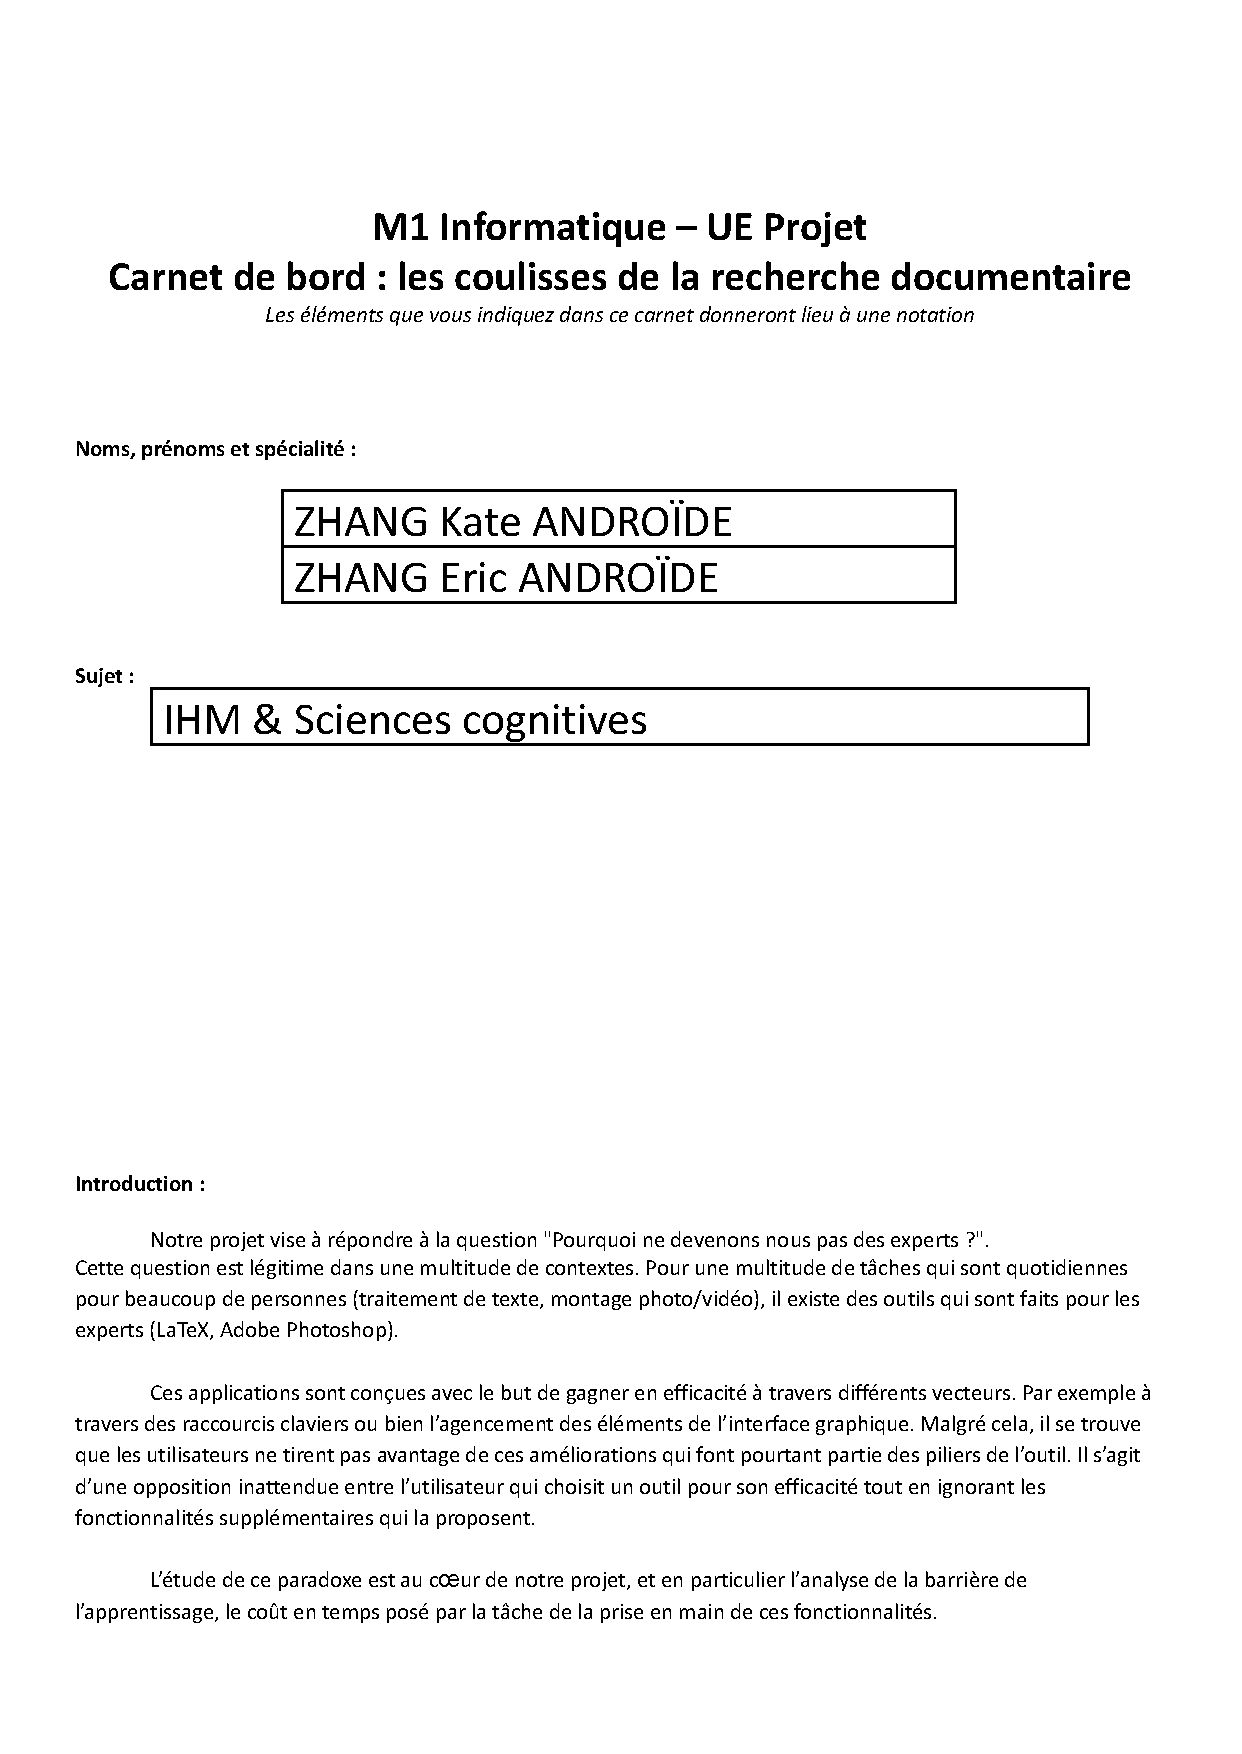
\includepdf[pages=-]{cdb.pdf}
\end{document}
